\documentclass{beamer}
\usepackage[ngerman]{babel}
\usepackage{booktabs}
\usepackage{tabulary}
\usepackage{siunitx}

\usetheme{imise}
\author{Konrad Höffner}
\date{2017-05-16, Institutskolloquium}
\title{Werkzeuge der SNIK Ontologie}
%\institute{IMISE Institutskolloquium}
\subtitle{\url{https://github.com/KonradHoeffner/latex/releases/download/colloquium/colloquium.pdf}}
\newcommand{\todo}[1]{TODO: #1}
\newcommand{\imageslide}[3][]
{
%\usebackgroundtemplate{\includegraphics[height=1.05\textheight]{#1}}
%\usebackgroundtemplate{\includegraphics[width=1.07\textwidth]{#1}}
\begin{frame}{#2}
\centering\includegraphics[width=1\textwidth,height=0.8\textheight,keepaspectratio]{#3}
\\#1
\end{frame}
%\usebackgroundtemplate{}
}

\AtBeginSection[]{
  \begin{frame}
  \vfill
  \centering
  \begin{beamercolorbox}[sep=8pt,center,shadow=false,rounded=true]{title}
    \usebeamerfont{title}\insertsectionhead\par%
  \end{beamercolorbox}
  \vfill
  \end{frame}
}

\begin{document}
\begin{frame}
\titlepage
\end{frame}

\section{Einführung}

\imageslide[\url{http://www.snik.eu} \url{http://5stardata.info}]{SNIK Projekt}{img/5star.png}

\begin{frame}{Einsatz}
\centering
\begin{tabular}{ll}
\toprule
\textbf{Ziel}	&\textbf{Zielgruppe}\\
\midrule
Lehre			&Lehrer und Studenten\\ 
Datenintegration	&Krankenhausleitung, CIO\\
Formalisierung		&Domänenexperten, Ontologen\\
\bottomrule
\end{tabular}
\end{frame}

\begin{frame}{Ziele}
\begin{enumerate}
\item Publizieren 
\item Visualisieren 
\item Evaluieren
\item Integrieren 
\end{enumerate}
\end{frame}

\section{Publizieren}

\imageslide[\url{https://github.com/IMISE/snik-ontology}]{RDF Dump}{img/rdfdump.png}
\imageslide[\url{https://protegewiki.stanford.edu/}]{RDF Dump in Protégé}{img/protege.png}
\imageslide[\url{http://www.snik.eu/sparql}]{SPARQL Endpoint}{img/sparqlresult.png}

\section{Visualisieren}

\imageslide[\url{http://www.snik.eu/ontology}]{RDF Browser---LodView}{img/browse-cio.png}

\imageslide[\url{http://www.snik.eu/graph}]{Graphvisualisierung I}{img/graph-entitytype.png}
\imageslide[\url{http://www.snik.eu/graph}]{Graphvisualisierung II}{img/graph-erf.png}
\imageslide[\url{http://www.snik.eu/graph}]{Graphvisualisierung---Kürzester Weg}{img/shortestpath.png}
\imageslide[\url{http://www.snik.eu/graph}]{Graphvisualisierung---Spiderworm}{img/spiderworm.png}


\begin{frame}{LodLive \& Relfinder}
\centering
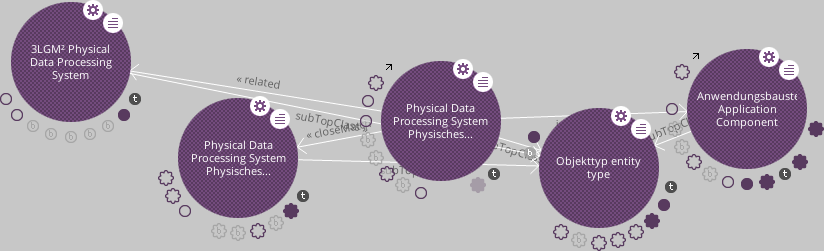
\includegraphics[width=\textwidth]{img/lodlive.png}\\
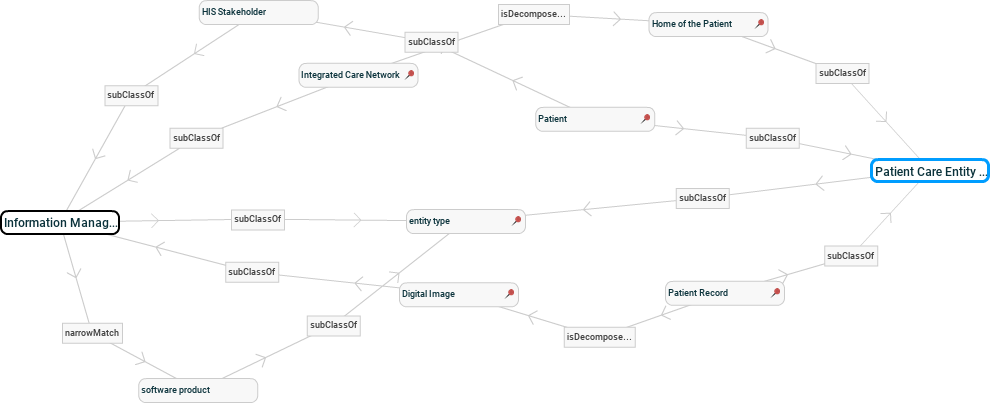
\includegraphics[width=\textwidth]{img/relfinder.png}
\end{frame}

\section{Evaluieren}

\imageslide[https://imise.github.io/snik-ontology/2017/04/12/dashboard]{Statistiken}{img/dashboard-medley.png}
\imageslide[\url{https://github.com/IMISE/snik-ontology/issues}]{Ticketsystem}{img/gitissue.png}
\imageslide[\url{http://www.snik.eu/evaluation}]{TripleCheckMate}{img/triplecheckmate.png}

\section{Integrieren}

\imageslide[\url{http://www.snik.eu/sparql}]{SPARQL Endpoint}{img/sparqlresult.png}

\imageslide[http://aksw.org/Projects/LIMES]{LIMES}{img/limes.png}

\iffalse
\begin{frame}{Interlinking}
\begin{itemize}
\item Verknüpfungen zwischen Klassen verschiedener Ontologien
\item LIMES Tool von AKSW um Axel Ngonga
\item Finden von Kandidaten durch Stringähnlichkeit, manuelle Verifizierung und Kategorisierung
\end{itemize}
\end{frame}
\fi

\imageslide[https://github.com/IMISE]{Öffentliche Softwarerepositories}{img/github.png}

\section{Überblick}

\begin{frame}
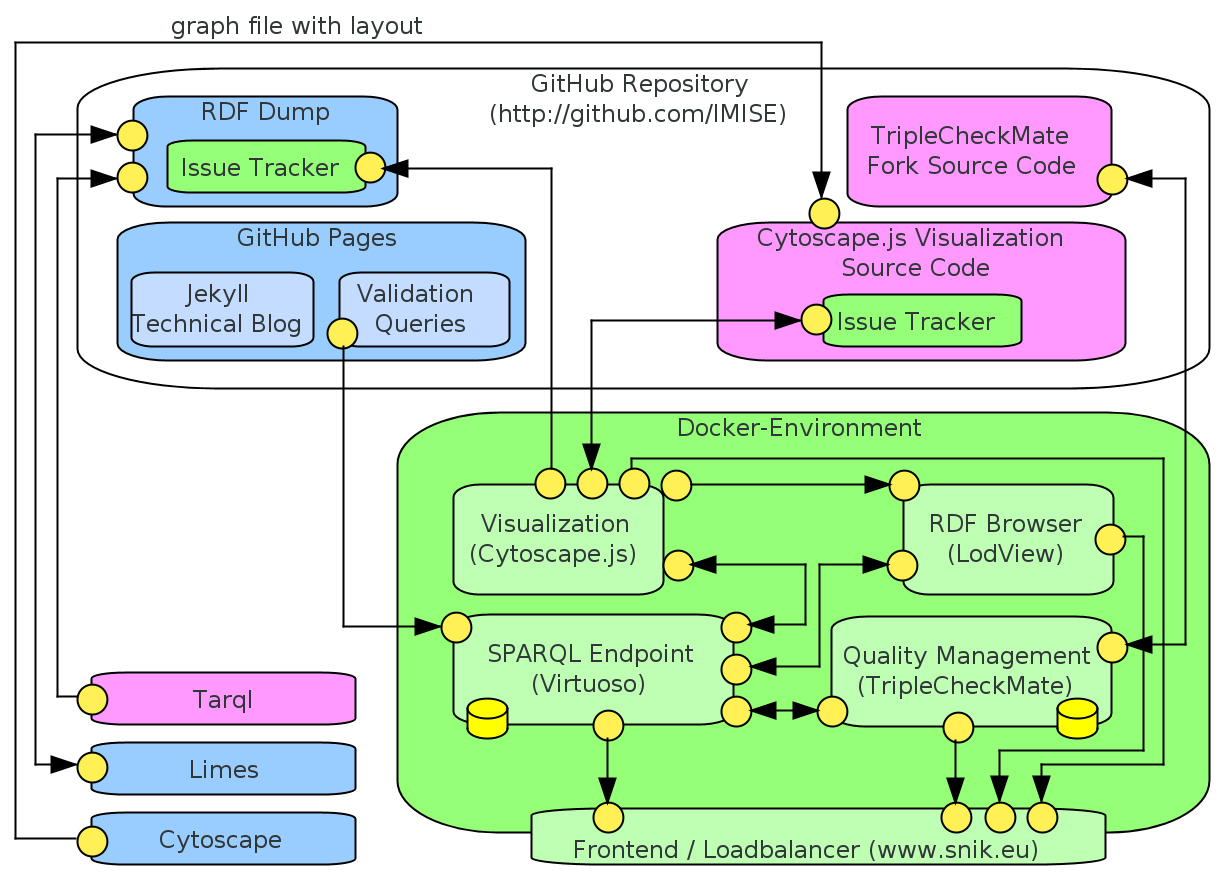
\includegraphics[width=\textwidth]{img/architecture.png}
\end{frame}

\begin{frame}[fragile]{Fragen?}
\begin{itemize}
\item Diese Präsentation \url{https://github.com/KonradHoeffner/latex/releases/download/colloquium/colloquium.pdf}
\vspace{0.5em}%here it works as intended
\item Überblick \url{http://www.snik.eu}
\item Visualisierung \url{http://www.snik.eu/graph}
\item SPARQL Endpunkt \url{http://www.snik.eu/sparql}
\item RDF Browser \url{http://www.snik.eu/ontology}
\item Evaluation \url{http://www.snik.eu/evaluation}
\item Twitter \url{https://twitter.com/snik\_proj}
\item Technisches Blog \url{https://imise.github.io/snik-ontology}
\item GitHub Organisation mit Ticketsystem \url{https://github.com/imise}
\end{itemize}
\end{frame}

\begin{frame}[fragile]{Externe Tools und Bibliotheken}
\begin{itemize}
\item LIMES Interlinker \url{http://aksw.org/Projects/LIMES}
\item Tarql Konvertierungstool \url{https://tarql.github.io/}
\item Cytoscape.js Graphbibliothek \url{http://js.cytoscape.org/}
\item Cytoscape Desktopvisualisierung \url{http://www.cytoscape.org/}
\end{itemize}
\end{frame}
 
\end{document}
